% ===================================================================
% Arquivo: capitulos/parte-III-pilares/cap-08-retificadoras.tex
% ===================================================================

\chapter{Funções de Ativação Retificadoras}
\label{cap:ativacao-retificadoras}

% ===================================================================
% Resumo do capítulo
% ===================================================================

\section{Exemplo Ilustrativo}

% ===================================================================
% ReLU
% ===================================================================

\section{Rectified Linear Unit e Revolução Retificadora}

\begin{equacaodestaque}{Rectified Linear Unit (ReLU)}
    \text{ReLU}(z_i) = \begin{cases}z_i, & \text{se } z_i > 0 \\0, & \text{se } z_i \leq 0\end{cases}
    \label{eq:relu}
\end{equacaodestaque}

\begin{figure}{h!}
        \centering
        \caption{Gráfico da função ReLU.}
        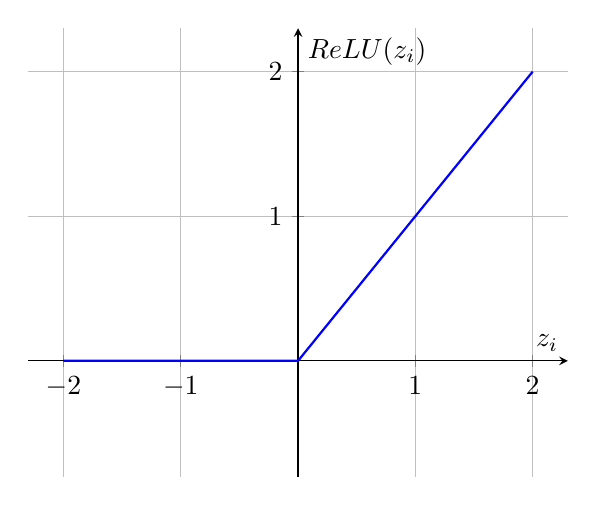
\begin{tikzpicture}
            \begin{axis}[
                xlabel={$z_i$},
                ylabel={$\text{ReLU}(z_i)$},
                xmin=-2.3, xmax=2.3,
                ymin=-0.8, ymax=2.3,
                axis lines=middle,
                grid=major,
            ]
            \addplot[blue, thick, domain=-2:2] {max(0, x)};
            \end{axis}
        \end{tikzpicture}
        \label{fig:relu}
\end{figure}

\begin{equacaodestaque}{Derivada Rectified Linear Unit (ReLU)}
    \frac{d}{dz_i} [ReLU](z_i) = \begin{cases}1, & \text{se } z_i > 0 \\0, & \text{se } z_i \leqslant 0 \end{cases}
    \label{eq:relu-derivada}
\end{equacaodestaque}

\begin{figure}[h!] % Use [htbp] para dar flexibilidade ao LaTeX
    \centering % Centraliza o gráfico na página
    \caption{Gráfico da Derivada da Função ReLU}
    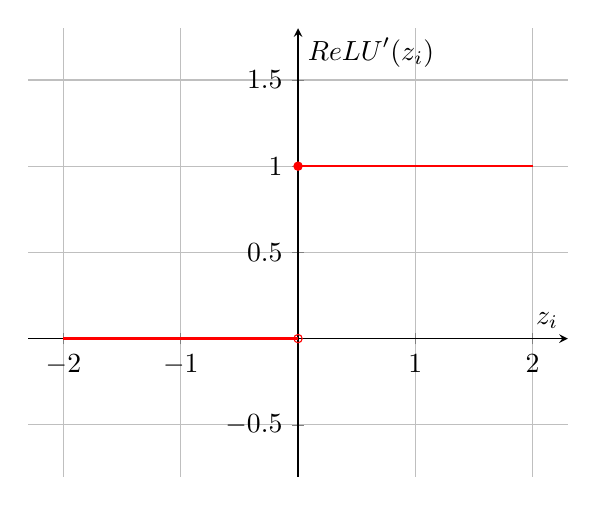
\begin{tikzpicture}
        \begin{axis}[
            xlabel={$z_i$},
            ylabel={$\text{ReLU}'(z_i)$},
            xmin=-2.3, xmax=2.3,
            ymin=-0.8, ymax=1.8,
            axis lines=middle,
            grid=major
        ]
        \addplot[red, thick, domain=-2:0] {0};
        \addplot[red, thick, domain=0:2] {1};
        \addplot[red, only marks, mark=o, mark size=1.5pt] coordinates {(0,0)};
        \addplot[red, only marks, mark=*, mark size=1.5pt] coordinates {(0,1)};
        \end{axis}
    \end{tikzpicture}
    \label{fig:relu-derivada}
\end{figure}

\subsection{Implementação em Python}

\begin{codelisting}{Classe completa do função de ativação Rectified Linear Unit}{gd_class}
import numpy as np
from layers.base import Layer

class ReLU(Layer):
    def __init__(self):
        super().__init__()
        self.input = None

    def forward(self, input_data):
        self.input = input_data
        return np.maximum(0, self.input)

    def backward(self, grad_output):
        relu_grad = (self.input > 0)

        # Apply the chain rule
        return grad_output * relu_grad, None
\end{codelisting}

\section{Dying ReLUs Problem}

\section{Corrigindo o Dying ReLUs Problem: As Variantes com Vazamento}

\subsection{Leaky ReLU}

\begin{equacaodestaque}{Leaky ReLU (LReLU)}
    \text{LReLU}(z_i) = \begin{cases}z_i, & \text{se } z_i \ge 0 \\ \alpha \cdot z_i, & \text{se } z_i < 0\end{cases}
    \label{eq:leaky-relu}
\end{equacaodestaque}

\begin{figure}[h!]
    \centering
    \caption{Gráfico da Função Leaky ReLU (LReLU) com $\alpha = 0.1$}
    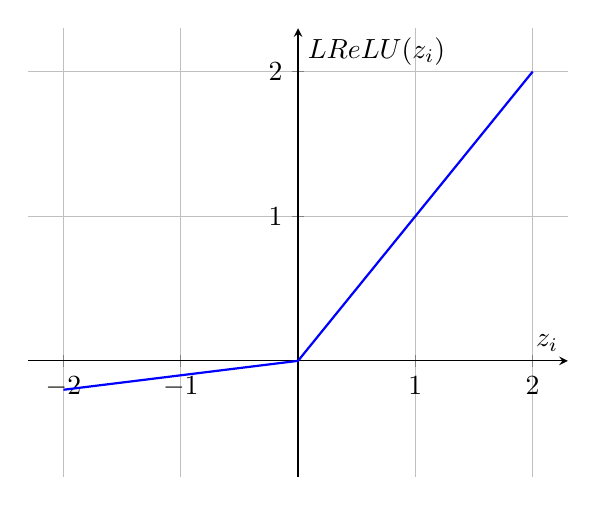
\begin{tikzpicture}
        \begin{axis}[
            xlabel={$z_i$},
            ylabel={$\text{LReLU}(z_i)$},
            xmin=-2.3, xmax=2.3,
            ymin=-0.8, ymax=2.3,
            axis lines=middle,
            grid=major,
        ]
        % \leakyalpha é o comando que você definiu no preâmbulo (0.1)
        \addplot[blue, thick, domain=-2:2] {x > 0 ? x : 0.1*x};
        \end{axis}
    \end{tikzpicture}
    \label{fig:leaky-relu}
\end{figure}

\begin{equacaodestaque}{Derivada Leaky ReLU (LReLU)}
    \frac{d}{dz_i} [LReLU](z_i) = \begin{cases}1, & \text{se } z_i > 0 \\ \alpha, & \text{se } z_i \leqslant  0 \end{cases}
    \label{eq:leaky-relu-derivada}
\end{equacaodestaque}

\begin{figure}[h!]
    \centering
    \caption{Gráfico da Derivada da Função Leaky ReLU (LReLU) com $\alpha = 0.1$}
    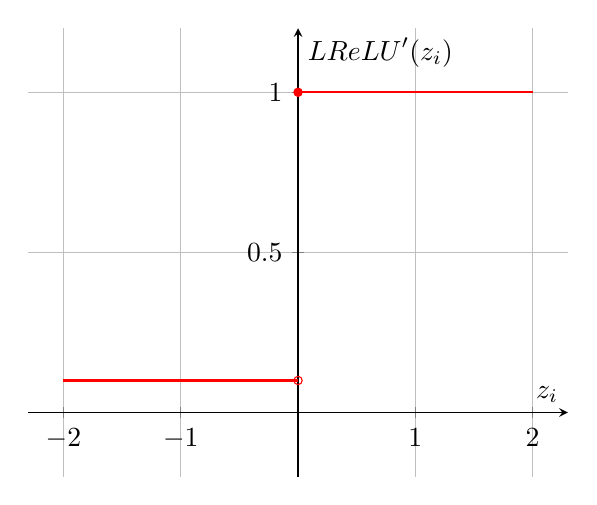
\begin{tikzpicture}
        \begin{axis}[
            xlabel={$z_i$},
            ylabel={$\text{LReLU}'(z_i)$},
            xmin=-2.3, xmax=2.3,
            ymin=-0.2, ymax=1.2,
            axis lines=middle,
            grid=major
        ]
        \def\alphaVal{0.1} % Define alpha for the derivative graph

        \addplot[red, thick, domain=-2:0] {\alphaVal};
        \addplot[red, thick, domain=0:2] {1};
        \addplot[red, only marks, mark=o, mark size=1.5pt] coordinates {(0,\alphaVal)};
        \addplot[red, only marks, mark=*, mark size=1.5pt] coordinates {(0,1)};
        \end{axis}
    \end{tikzpicture}
    \label{fig:leaky-relu-derivada}
\end{figure}

\subsubsection{Implementação em Python}

\begin{codelisting}{Classe completa do função de ativação Leaky ReLU}{gd_class}
import numpy as np
from layers.base import Layer


class LeakyReLU(Layer):
    def __init__(self, alpha=0.01):
        super().__init__()
        self.input = None
        self.alpha = alpha

    def forward(self, input_data):
        self.input = input_data
        return np.maximum(self.input * self.alpha, self.input)

    def backward(self, grad_output):
        leaky_relu_grad = np.where(self.input > 0, 1, self.alpha)
        return grad_output * leaky_relu_grad, None
\end{codelisting}

\subsection{Parametric ReLU}

\begin{equacaodestaque}{Parametric ReLU (PReLU)}
    \text{PReLU}(z_i) = \begin{cases}z_i, & \text{se } z_i \ge 0 \\ \alpha_i \cdot z_i, & \text{se } z_i < 0\end{cases}
    \label{eq:prelu}
\end{equacaodestaque}

\begin{figure}[h!]
    \centering
    \caption{Gráfico da Função Parametric ReLU (PReLU) com $\alpha=0.2$}
    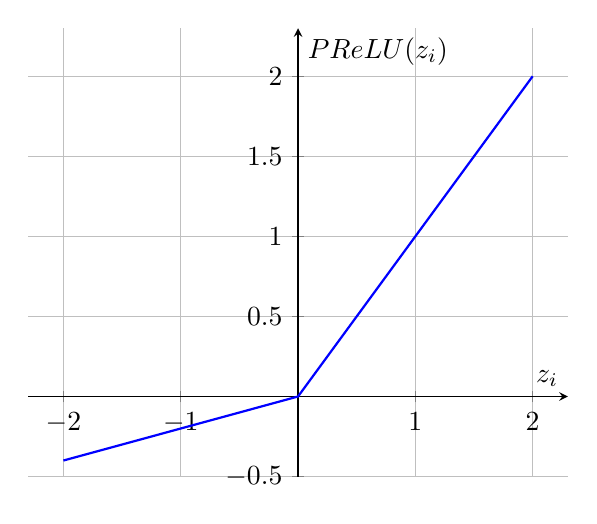
\begin{tikzpicture}
        \begin{axis}[
            xlabel={$z_i$},
            ylabel={$\text{PReLU}(z_i)$},
            xmin=-2.3, xmax=2.3,
            ymin=-0.5, ymax=2.3,
            axis lines=middle,
            grid=major,
        ]
        % Define um valor exemplo de alpha para o gráfico
        \def\alphaVal{0.2} 
        \addplot[blue, thick, domain=-2:2] {x >= 0 ? x : \alphaVal*x};
        \end{axis}
    \end{tikzpicture}
    \label{fig:prelu}
\end{figure}

\begin{equacaodestaque}{Derivada Parametric ReLU (PReLU)}
    \frac{d}{dz_i} [PReLU](z_i) = \begin{cases}1, & \text{se } z_i > 0 \\ \alpha_i, & \text{se } z_i < 0 \\ \nexists, & \text{se } z_i = 0\end{cases}
    \label{eq:prelu-derivada}
\end{equacaodestaque}

\begin{figure}[h!]
    \centering
    \caption{Gráfico da Derivada da Função Parametric ReLU (PReLU) com ($\alpha=0.2$)}
    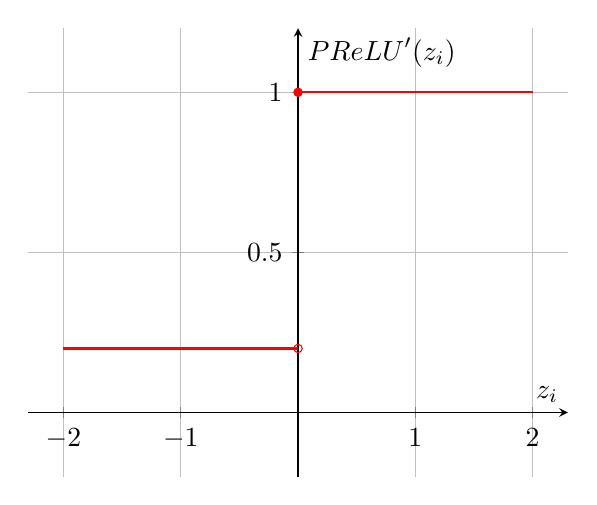
\begin{tikzpicture}
        \begin{axis}[
            xlabel={$z_i$},
            ylabel={$\text{PReLU}'(z_i)$},
            xmin=-2.3, xmax=2.3,
            ymin=-0.2, ymax=1.2,
            axis lines=middle,
            grid=major
        ]
        % Define um valor exemplo de alpha para o gráfico
        \def\alphaVal{0.2}

        \addplot[red, thick, domain=-2:0] {\alphaVal};
        \addplot[red, thick, domain=0:2] {1};
        \addplot[red, only marks, mark=o, mark size=1.5pt] coordinates {(0,\alphaVal)};
        \addplot[red, only marks, mark=*, mark size=1.5pt] coordinates {(0,1)};
        \end{axis}
    \end{tikzpicture}
    \label{fig:prelu-derivada}
\end{figure}

\subsection{Randomized Leaky ReLU}

\begin{equacaodestaque}{Randomized Leaky ReLU (RReLU)}
    \text{RReLU}(z_i) = \begin{cases} z_i, & \text{se } z_i > 0 \\ \alpha_i z_i, & \text{se } z_i \leq 0 \end{cases}
    \label{eq:rrelu}
\end{equacaodestaque}

\begin{figure}[h!]
    \centering
    \caption{Gráfico da Função Randomized Leaky ReLU (RReLU) com Diferentes Inclinações Aleatórias para a Parte Negativa}
    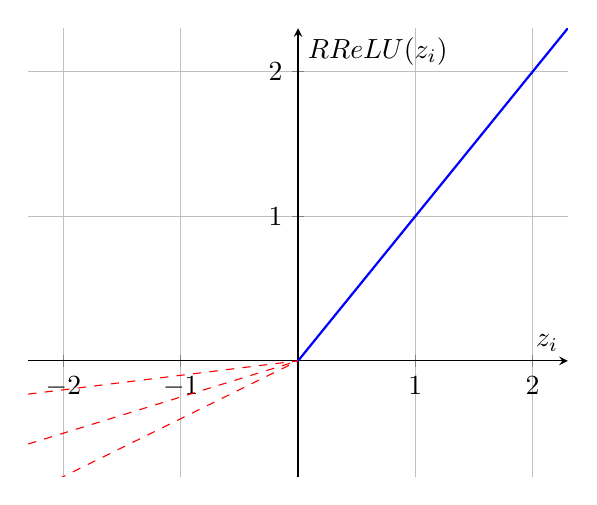
\begin{tikzpicture}
        \begin{axis}[
            xlabel={$z_i$},
            ylabel={$\text{RReLU}(z_i)$},
            xmin=-2.3, xmax=2.3,
            ymin=-0.8, ymax=2.3,
            axis lines=middle,
            grid=major,
            legend pos=north west,
            legend style={font=\tiny}
        ]
        \addplot[blue, thick, domain=0:2.3] {x};
        \addplot[red, dashed, domain=-2.3:0, samples=2] {0.1*x};
        \addplot[red, dashed, domain=-2.3:0, samples=2] {0.25*x};
        \addplot[red, dashed, domain=-2.3:0, samples=2] {0.4*x};
        \end{axis}
    \end{tikzpicture}
    \label{fig:rrelu}
\end{figure}

\begin{equacaodestaque}{Derivada Randomized Leaky ReLU (RReLU)}
    \frac{d}{dz_i} [RReLU](z_i) = \begin{cases}1, & \text{se } z_i > 0 \\ \alpha_i, & \text{se } z_i \leqslant  0 \end{cases}
    \label{eq:rrelu-derivada}
\end{equacaodestaque}

\begin{figure}[h!]
    \centering
    \caption{Gráfico da Derivada da Função Randomized Leaky ReLU (RReLU) com $l=0.1, u=0.3$}
    \begin{tikzpicture}
        \begin{axis}[
            xlabel={$z_i$},
            ylabel={$\text{RReLU}'(z_i)$},
            xmin=-2.3, xmax=2.3,
            ymin=-0.2, ymax=1.2,
            axis lines=middle,
            grid=major,
            legend pos=north west,
            legend style={font=\scriptsize}
        ]
        % Define l e u para a distribuição uniforme U(l,u)
        \def\lVal{0.1}
        \def\uVal{0.3}

        % Plota a derivada para z > 0
        \addplot[red, thick, domain=0:2.1] {1};
        \addlegendentry{$f'(z_i) = 1$}

        % Plota a região hachurada para z < 0
        \addplot[
            pattern=north east lines, 
            pattern color=blue!50,
            draw=none
        ] coordinates {(-2.1, \lVal) (0, \lVal) (0, \uVal) (-2.1, \uVal)} -- cycle;
        \addlegendentry{$\alpha_i \sim U(l,u)$}

        % Marcadores na descontinuidade
        \addplot[blue, only marks, mark=o, mark size=1.5pt, forget plot] coordinates {(0,\lVal)};
        \addplot[blue, only marks, mark=o, mark size=1.5pt, forget plot] coordinates {(0,\uVal)};
        \addplot[red, only marks, mark=*, mark size=1.5pt, forget plot] coordinates {(0,1)};
        
        \end{axis}
    \end{tikzpicture}
    \label{fig:rrelu-derivada}
\end{figure}

\section{Em Busca da Suavidade}

\subsection{Exponential Linear Unit}

\begin{equacaodestaque}{Exponential Linear Unit (ELU)}
    \text{ELU}(z_i) = \begin{cases}z_i, & \text{se } z_i \ge 0 \\ \alpha \cdot (e^{z_i} - 1), & \text{se } z_i < 0\end{cases}
    \label{eq:elu}
\end{equacaodestaque}


\begin{figure}[h!]
    \centering
    \caption{Gráfico da Função Exponential Linear Unit (ELU) com $\alpha=1$}
    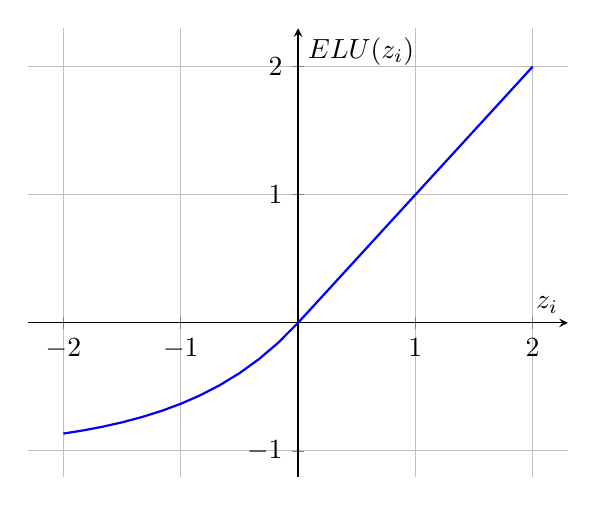
\begin{tikzpicture}
        \begin{axis}[
            xlabel={$z_i$},
            ylabel={$\text{ELU}(z_i)$},
            xmin=-2.3, xmax=2.3,
            ymin=-1.2, ymax=2.3,
            axis lines=middle,
            grid=major,
        ]
        % Define alpha para o gráfico. O valor comum para ELU é 1.
        \def\alphaVal{1} 
        \addplot[blue, thick, domain=-2:2] {x >= 0 ? x : \alphaVal*(exp(x) - 1)};
        \end{axis}
    \end{tikzpicture}
    \label{fig:elu}
\end{figure}

\begin{equacaodestaque}{Derivada Exponential Linear Unit (ELU)}
    \frac{d}{dz_i} [ELU](z_i) = \begin{cases}1, & \text{se } z_i > 0 \\ \alpha \cdot e^{z_i}, & \text{se } z_i \le 0 \end{cases}
    \label{eq:elu-derivada}
\end{equacaodestaque}

\begin{figure}[h!]
    \centering
    \caption{Gráfico da Derivada da Função Exponential Linear Unit (ELU) com $\alpha=1$}
    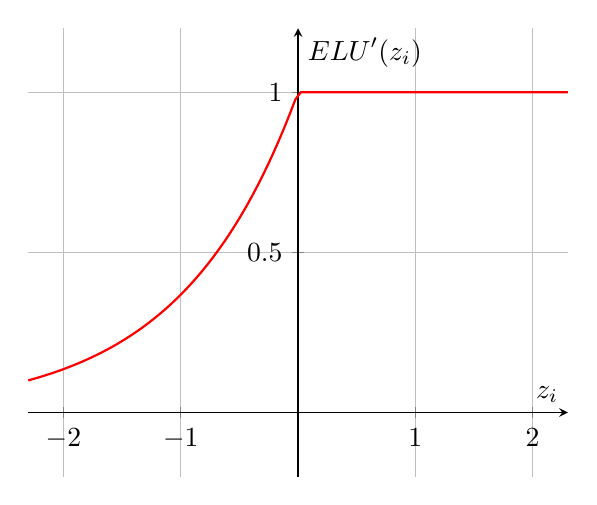
\begin{tikzpicture}
        \begin{axis}[
            xlabel={$z_i$},
            ylabel={$\text{ELU}'(z_i)$},
            xmin=-2.3, xmax=2.3,
            ymin=-0.2, ymax=1.2,
            axis lines=middle,
            grid=major
        ]
        % Define alpha para o gráfico
        \def\alphaVal{1} 

        % Plota a derivada usando uma única expressão condicional
        \addplot[red, thick, domain=-2.3:2.3, samples=100] {x > 0 ? 1 : \alphaVal*exp(x)};
        
        \end{axis}
    \end{tikzpicture}
    \label{fig:elu-derivada}
\end{figure}

\subsection{Scaled Exponential Linear Unit}

\begin{equacaodestaque}{Scaled Exponential Linear Unit (ELU)}
    \text{SELU}(z_i) = \lambda \begin{cases}z_i, & \text{se } z_i > 0 \\ \alpha \cdot (e^{z_i} - 1), & \text{se } z_i \le 0\end{cases}
    \label{eq:selu}
\end{equacaodestaque}

\begin{figure}[h!]
    \centering
    \caption{Gráfico da Função Scaled Exponential Linear Unit (SELU) com $\alpha \approx 1.67 e \lambda \approx 1.05$}
    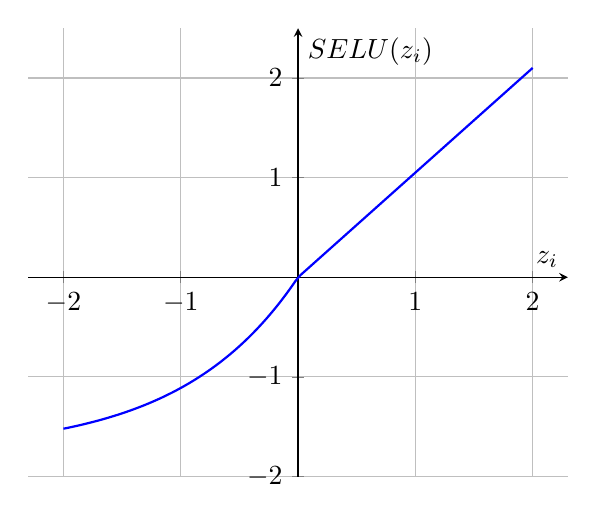
\begin{tikzpicture}
        \begin{axis}[
            xlabel={$z_i$},
            ylabel={$\text{SELU}(z_i)$},
            xmin=-2.3, xmax=2.3,
            ymin=-2, ymax=2.5,
            axis lines=middle,
            grid=major,
        ]
        % Define as constantes da SELU para o gráfico
        \def\alphaVal{1.67326}
        \def\lambdaVal{1.0507}
        \addplot[blue, thick, domain=-2:2, samples=100] {x > 0 ? \lambdaVal*x : \lambdaVal*\alphaVal*(exp(x) - 1)};
        \end{axis}
    \end{tikzpicture}
    \label{fig:selu}
\end{figure}

\begin{equacaodestaque}{Derivada Scaled Exponential Linear Unit (ELU)}
    \frac{d}{dz_i} [SELU](z_i) = \lambda \begin{cases}1, & \text{se } z_i > 0 \\ \alpha \cdot e^{z_i}, & \text{se } z_i \le 0\end{cases}
    \label{eq:selu-derivada}
\end{equacaodestaque}

\begin{figure}[h!]
    \centering
    \caption{Gráfico da Derivada da Função Scaled Exponential Linear Unit (SELU) com $\alpha \approx 1.67, \lambda \approx 1.05$}
    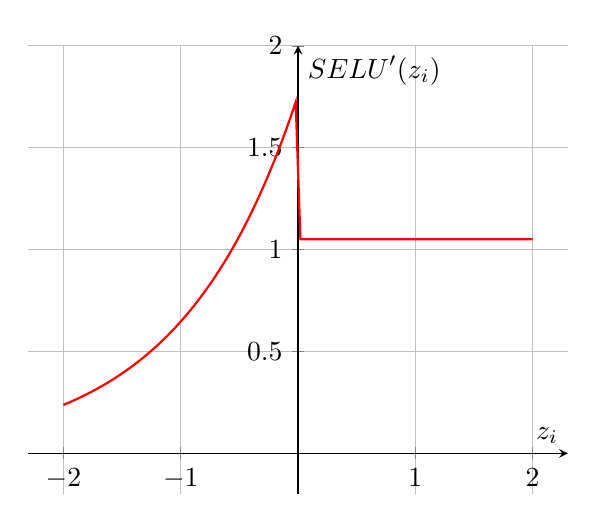
\begin{tikzpicture}
        \begin{axis}[
            xlabel={$z_i$},
            ylabel={$\text{SELU}'(z_i)$},
            xmin=-2.3, xmax=2.3,
            ymin=-0.2, ymax=2.0, % Ajustado para lambda > 1
            axis lines=middle,
            grid=major
        ]
        % Define as constantes da SELU para o gráfico
        \def\alphaVal{1.67326}
        \def\lambdaVal{1.0507}

        \addplot[red, thick, domain=-2:2, samples=100] {x > 0 ? \lambdaVal*1 : \lambdaVal*\alphaVal*exp(x)};
        \end{axis}
    \end{tikzpicture}
    \label{fig:selu-derivada}
\end{figure}

\subsection{Noisy ReLU}

\begin{equacaodestaque}{Noisy ReLU (NReLU)}
    \text{NReLU}(z_i) = \begin{cases} 
    0 & \text{se } z_i \le 0 \\ 
    z_i + \mathcal{N} (0, \sigma(z_i)) & \text{se } z_i > 0 
    \end{cases}
    \label{eq:nrelu}
\end{equacaodestaque}

\begin{figure}[h!]
    \centering
    \caption{Gráfico da Função Noisy ReLU (NReLU)}
    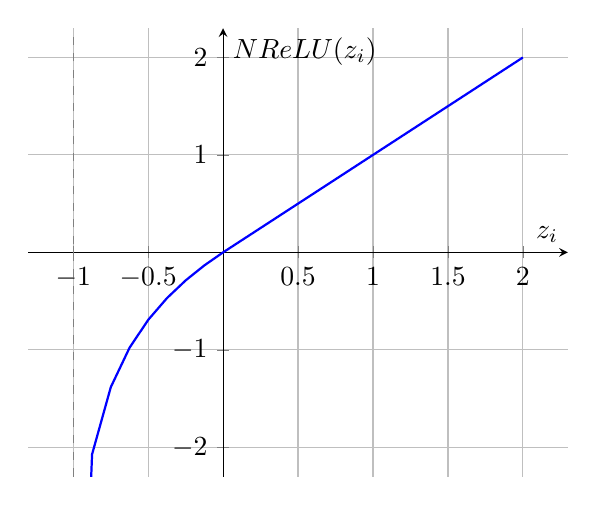
\begin{tikzpicture}
        \begin{axis}[
            xlabel={$z_i$},
            ylabel={$\text{NReLU}(z_i)$},
            xmin=-1.3, xmax=2.3,
            ymin=-2.3, ymax=2.3,
            axis lines=middle,
            grid=major,
            domain=-0.999:2, % Domínio para evitar o log de zero ou negativo
        ]
        % A função ln(1+x) está definida para x > -1
        \addplot[blue, thick] {x >= 0 ? x : ln(1+x)};
        % Linha vertical para mostrar a assíntota em z = -1
        \draw[dashed, gray] (axis cs:-1, -2.3) -- (axis cs:-1, 2.3);
        \end{axis}
    \end{tikzpicture}
    \label{fig:nrelu}
\end{figure}

\begin{equacaodestaque}{Derivada Noisy ReLU (NReLU)}
    \frac{d}{dz_i}[\text{NReLU}](z_i) = \begin{cases} 
    0 & \text{se } z_i \le 0 \\ 
    1 & \text{se } z_i > 0 
    \end{cases}
    \label{eq:nrelu-derivada}
\end{equacaodestaque}

\begin{figure}[htbp] % Use [htbp] para dar flexibilidade ao LaTeX
    \centering % Centraliza o gráfico na página
    \caption{Gráfico da função Backward Pass da Noisy ReLU}
    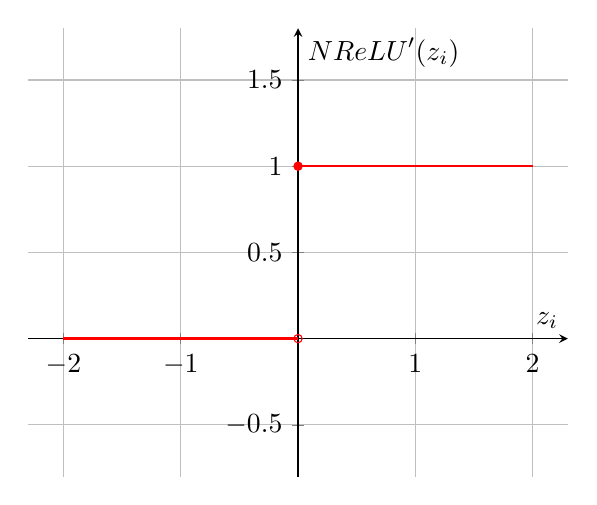
\begin{tikzpicture}
        \begin{axis}[
            xlabel={$z_i$},
            ylabel={$\text{NReLU}'(z_i)$},
            xmin=-2.3, xmax=2.3,
            ymin=-0.8, ymax=1.8,
            axis lines=middle,
            grid=major
        ]
        \addplot[red, thick, domain=-2:0] {0};
        \addplot[red, thick, domain=0:2] {1};
        \addplot[red, only marks, mark=o, mark size=1.5pt] coordinates {(0,0)};
        \addplot[red, only marks, mark=*, mark size=1.5pt] coordinates {(0,1)};
        \end{axis}
    \end{tikzpicture}
    \label{fig:nrelu-derivada}
\end{figure}

\section{O Problema dos Gradientes Explosivos}

\section{Comparativo de Desempenho das Funções Retificadoras}